\documentclass[../main.tex]{subfiles}
 
\begin{document}

\newpage

\section{Introduction and overview}
\label{intro}

The HDF5 Subfiling \Gls{VFD} is an MPI-based File Driver that was introduced in the HDF5 1.14.0 release.
This File Driver allows an HDF5 application to create HDF5 files which are distributed across a collection
of "\textit{subfiles}" in equal-sized data segment "\textit{stripes}." I/O to the logical HDF5 file is directed to the
appropriate "\textit{subfile}" according to the Subfiling VFD configuration and a system of "\textit{I/O Concentrators}."
For more information on the general design of this VFD, refer to the \href{https://github.com/HDFGroup/hdf5doc/blob/master/RFCs/HDF5_Library/VFD_Subfiling/RFC_VFD_subfiling_200424.docx}{Subfiling RFC}.

By allowing a user to configure its various parameters, such as the data stripe size, number of subfiles,
etc., the Subfiling VFD aims to enable an HDF5 application to achieve a middle ground between the single
shared file and file-per-process approaches to parallel file I/O for a particular machine that the application
is running on. In general, the goal is to enable these applications to avoid some of the complexity of the
file-per-process approach while also minimizing locking issues that can occur on a parallel file system
with the single shared file approach at large scales.

The Subfiling feature consists of two major components: the Subfiling VFD and an underlying I/O
Concentrator VFD. The Subfiling VFD is responsible for managing Subfiling metadata and configuration
information, as well as breaking down I/O requests into the appropriate offset/length pairs based on
the Subfiling configuration and forwarding those requests to an I/O Concentrator VFD that is stacked
under the Subfiling VFD. The I/O Concentrator VFD is responsible for receiving I/O offset/length
pairs from the Subfiling VFD and forwarding each of these I/O requests to the I/O Concentrator
(typically, an MPI rank/dedicated thread/etc.) that is controlling the relevant portion of the logical
HDF5 file.

The Subfiling feature was designed to allow different types of I/O Concentrator VFDs in the future,
but currently includes a reference implementation of an I/O Concentrator VFD (called the
"IOC VFD"), which controls a dedicated set of MPI ranks acting as I/O Concentrators. Each of those MPI
ranks hosts an I/O thread pool and uses POSIX I/O calls (e.g., pread/pwrite) within those I/O threads.
Figure \ref{fig:architecture} graphically presents the current architecture of the Subfiling feature.

\begin{figure}
\centering
\scalebox{.9}{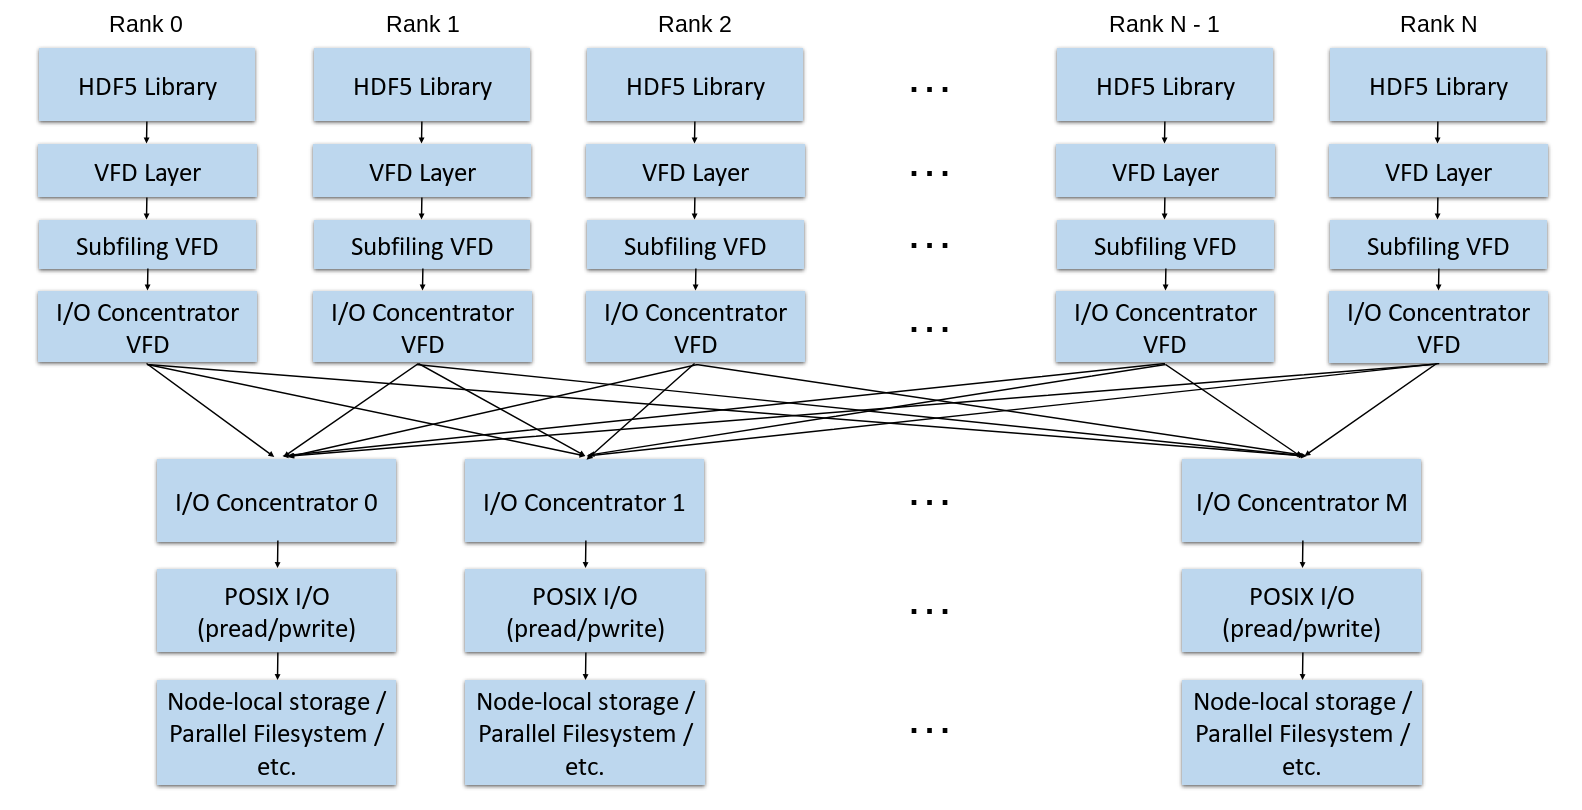
\includegraphics[width=\textwidth]{images/Subfiling Architecture.png}}
\caption{Subfiling feature architecture overview}
\label{fig:architecture}
\end{figure}

When an HDF5 file is written with the Subfiling VFD, several different files are created: The HDF5
stub file, a Subfiling configuration file and the various subfiles. For example, an HDF5 file called
"outFile.h5" is created with the Subfiling VFD, along with four subfiles, Figure \ref{fig:outputs}.

\begin{figure}
\centering
\scalebox{.8}{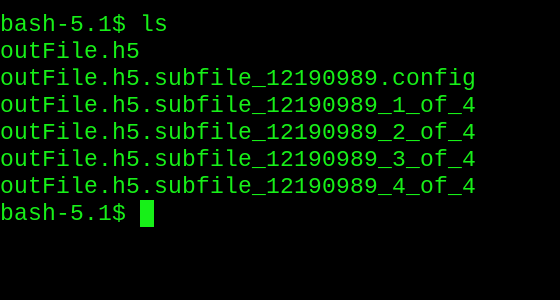
\includegraphics[width=\textwidth]{images/Subfiling components.png}}
\caption{Subfiling feature output files}
\label{fig:outputs}
\end{figure}

The first of these files, the HDF5 stub file, looks like a standard HDF5 file but only contains a small
portion of the file's metadata and is primarily used for HDF5 to determine when a file was written with
the Subfiling VFD.

The next file created is a Subfiling configuration file. The Subfiling VFD keeps track of its configuration
by writing it into the previously mentioned HDF5 stub file as metadata. However, this configuration information
also gets written out to a Subfiling configuration file so external tools can obtain that information
and access Subfiling VFD-based HDF5 files without needing to involve HDF5. An example of the Subfiling
configuration file is presented in Figure \ref{fig:config_file}.

\begin{figure}
\centering
\scalebox{.8}{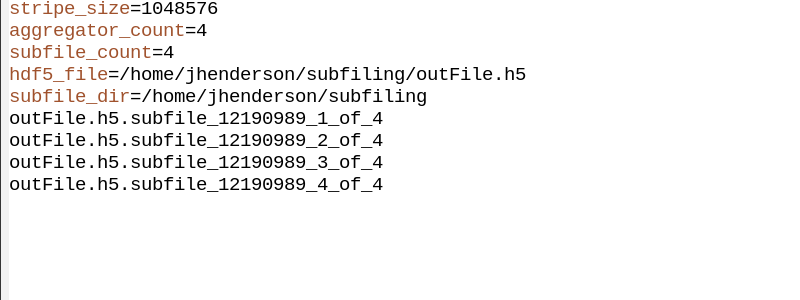
\includegraphics[width=\textwidth]{images/Subfiling Config File.png}}
\caption{Subfiling configuration file}
\label{fig:config_file}
\end{figure}

Finally, the created subfiles (\texttt{outFile.h5.subfile\_12190989\_X\_of\_4}) simply contain
the raw file data, distributed in a round-robin fashion across the subfiles according to the Subfiling
stripe size.
 
\end{document}